\chapter{Caso de Uso} \label{ch:cdu}

O presente capítulo visa explicar o caso de uso da ontologia. O caso de uso da
ontologia é uma simulação de uma casa em sua vida cotidiana normal, isto é, os
personagens vão para escola, trabalho, fazem compras e ficam em casa.
Entretanto, antes desse caso de uso ser abordado na seção~\ref{ch:cdu:svc}
será falado como a ontologia foi testada juntamente com a plataforma \jason.
A seção~\ref{ch:cdu:tbc} explica as ferramentas desenvolvidas para testar a base
de crenças e, consequentemente, a ontologia. Elas são duas uma interativa e
outra não interativa que serve como uma especie de teste unitário.

\section{Teste da Base de Crenças} \label{ch:cdu:tbc}

Os testes da base de crenças tem como finalidade checar se a utilização normal
esta acontecendo da maneira esperada. Assim, eles fazem testes de inserção,
recuperação, remoção e listagem. A listagem é feita implementando a interface
\emph{Iterable} da plataforma Java e é usada, principalmente, quando a
interface gráfica da plataforma \jason esta em modo depuração e
exibindo a base de crenças.

\begin{figure}
	\begin{center}
		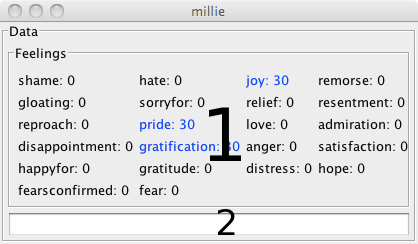
\includegraphics[width=70mm]{figuras/introductionDF.png}
	\end{center}
	\caption{Interface para mostrar os sentimentos dos agentes.}
	\label{fig:introducaoDF}
\end{figure}

A primeira aplicação de teste desenvolvida foi de maneira interativa conforme
pode ser observado na Figura~\ref{fig:introducaoDF}. A aplicação permite que o
usuário escreva as crenças do agente em um campo texto (área 2 na figura) e
esse é enviado diretamente para a base de crença do agente. A área 1 na mesma
figura é utilizada para demostrar a valência das emoções.
Essas informações podem aparecer em: preto, se não houve alteração com o ciclo
anterior; azul, se houve um aumento; vermelho, se houve uma diminuição do
valor.

\begin{figure}
	\begin{center}
		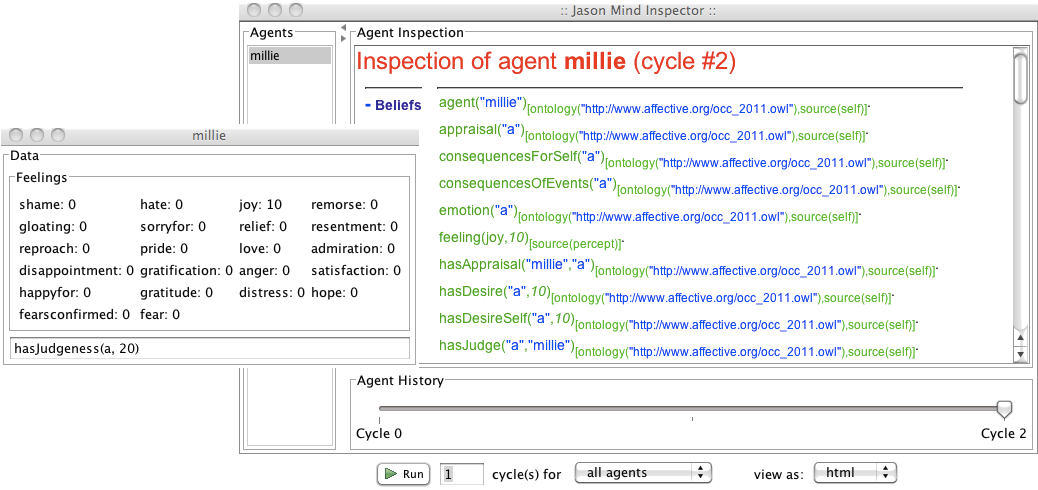
\includegraphics[width=150mm]{figuras/beforeLastInsertionOfPride.png}
		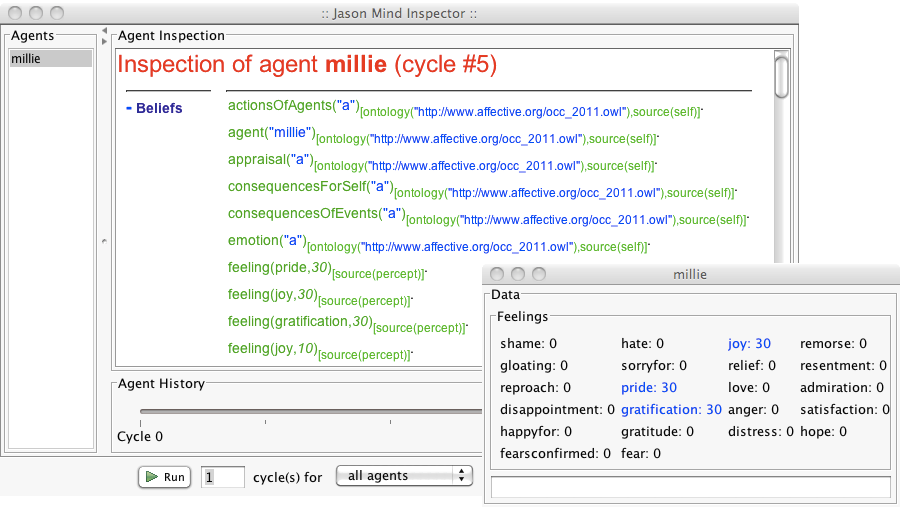
\includegraphics[width=150mm]{figuras/afterLastInsertionOfPride.png}
	\end{center}
	\caption{Exemplo de utilização criando uma emoção de orgulho.}
	\label{fig:testeJasonIntBase}
\end{figure}

Na Figura~\ref{fig:testeJasonIntBase} estão representados dois momentos da
criação de uma emoção de orgulho da parte do usuário. Na parte de cima, o
agente tem configurado uma avaliação de e sobre si próprio. Além disso, a
avaliação tem probabilidade nula ou irrelevante e o desejo para si mesmo foi
considerado com o valor 10. Esse valor poderia ser qualquer número inteiro,
mas se fosse negativo ao invés de alegria (\emph{joy}) o resultado atual seria
sofrimento (\emph{distress}). No campo de texto, o usuário irá inserir a
última relação para ser construída a percepção de orgulho.

Na parte de baixo da Figura~\ref{fig:testeJasonIntBase} pode se ver o
resultado obtido para a inserção da última crença. Conforme pode ser visto,
foi necessário três ciclos deliberativos para o agente ter a percepção do
sentimento. Na verdade, essa percepção não veio de um novo ciclo de simulação
rodando e sim que o agente acrescentou uma nova crença dizendo que havia um
passo novo então foi feita a avaliação das emoções quanto a necessidade de
se criar a percepção afetiva. Se fosse um passo normal da simulação, não se
teria na base de crenças duas percepções \emph{feeling} sobre uma emoção
porque a todo novo passo as percepções são limpas.

Na Listagem~\ref{lst:testeJasonIntBase} pode ser observado uma configuração
para se rodar a apresente aplicação\footnote{Veja a seção
\ref{sec-jason-overview} na página~\pageref{sec-jason-overview}
para ver uma introdução sobre esse tipo de arquivo.}. O ambiente na linha 4
espera que todos os agentes (configurados inicialmente no parâmetro 3) mandem
uma ação para prosseguir. O simulador espera pelo tempo (em milissegundos)
configurado no primeiro parâmetro por essas ações, caso não venha ignora o
agente e segue para o próximo ciclo. O segundo parâmetro permite que seja
configura um número que representa o último passo de simulação e no quarto
parâmetro permite configurar se uma segunda ação enviada no mesmo passo de
simulação é para ser enfileirada ou resultar em erro (essa é a opção atual).

\begin{center}
    \begin{minipage}{130mm}
	\lstset{linewidth=130mm}
	\lstinputlisting[frame=trbl, caption=Arquivo de projeto do \jason para a
aplicação interativa de teste, label=lst:testeJasonIntBase]{../../sampletConsole/eoaus.mas2j}
    \end{minipage}
\end{center}

A agente millie configurada da linha 7 à 11 utiliza opções do \jason para
alterar a base de crença sendo utilizada (\emph{beliefBaseClass}),
arquitetura do agente (\emph{agentArchClass}) e o próprio agente
(\emph{agentClass}). Dessas alterações, a mudança da base de crença e da
classe do agente foram explicadas na seção~\ref{ch:p:ipjo}\todo{garantir isso
depois}. Assim, para o presente exemplo a mudança da arquitetura na linha 9
foi realizada para criar e atualizar a janela que exibe os dados emotivos.

Cabe chamar a atenção que na linha 8 da Listagem~\ref{lst:testeJasonIntBase}
foi usada a ontologia afetiva desenvolvida somente. Assim, para o agente
utilizar as emoções ainda é necessário incluir as configurações do valor
excedido para se ter a emoção presente via código do agente. Uma amostra do
código utilizado para se fazer isso pode ser vista na
Listagem~\ref{lst:testeJasonIntSetup} e todo o código pode ser visto no
Anexo~X\todo{referencia e pagina}.

\lstset{linewidth=80mm}
\begin{wrapfigure}{l}{90mm}
	\begin{lstlisting}[frame=trbl,
caption=Parte do código do agente para aplicação interativa de teste,
label=lst:testeJasonIntSetup]
step(0)[source(percept),source(self)].

agent(millie).

hasSetup(millie, setup1).
hasThreshold(setup1, 0).
hasThresholdType(setup1, "Joy").

hasSetup(millie, setup2).
hasThreshold(setup2, 0).
hasThresholdType(setup2, "Distress").
	\end{lstlisting}
\end{wrapfigure}

A Listagem~\ref{lst:testeJasonIntSetup} mostra crenças que o agente terá
no inicio da simulação na plataforma \jason. Essas são populadas na memória
de acordo com a classe especificada na linha 8 da
Listagem~\ref{lst:testeJasonIntBase}. Esse processo já foi explicado na
seção~\ref{ch:p:ipjo}\todo{garantir isso}, a crença de \emph{step} como não
consta na ontologia será carregada na base de crenças padrão do \jason e as
demais mostradas serão inseridas na ontologia. Como pode ser observado, esse
processo é bastante transparente para o usuário.

Note também que o usuário precisou definir o limite para uma emoção virar
sentimento. No exemplo esse valor esta sendo definido como zero para que a
potência e a valência sejam iguais. Se for definido algum outro valor, a
potência será o valor total da emoção e esse valor não é de conhecimento do
agente. Ele conhece apenas a valência que será a diferença do valor total
menos o limite para ativação definido pela relação \emph{hasThreshold}. Por
exemplo, se o limite da pena (\emph{sorryFor}) é 6 e o valor atual é 8 então o
agente terá o sentimento com o valor 2 que será expresso por uma crença da
seguinte forma ``feeling("sorryFor",2).''.

%%%% fim da explicacao da aplicação interativa %%%%%

\begin{center}
    \begin{minipage}{140mm}
	\lstset{linewidth=140mm}
	\lstinputlisting[frame=trbl, caption=Arquivo de projeto do \jason para a
aplicação não interativa de teste,
label=lst:testeJasonNIBase]{../../sampletSummary/eoaus.mas2j}
    \end{minipage}
\end{center}

A aplicação não interativa utiliza a Listagem~\ref{lst:testeJasonNIBase} para
configurar o seu projeto. O ambiente especificado na linha 4 possui os mesmos
parâmetros do anterior com o acréscimo de um novo que indica uma ontologia.
Essa ontologia serve para o ambiente conhecer as rotinas dos agentes na
simulação, como deve ser desenhado o mapa exibido e as posições iniciais dos
agentes. O agente millie aqui é o utilizado para os testes e os limiares de
ativação de emoção estão configurados para valores diferentes. Existe uma
variedade de testes para as propriedades de objeto ou de dados e para as
instâncias de classes, além de testes das conclusões esperadas pela ontologia.
Veja o anexo~X\todo{botar o xodigo} para ver o código do agente.

\section{Simulando a Vida Cotidiana} \label{ch:cdu:svc}
\todo{era ``Simulando a Vida Cotidiana'' sem nada escrito}

...


